\documentclass[a4paper,12pt,twoside]{ThesisStyle}
\usepackage[utf8]{inputenc}
\usepackage{thesis-style}
\usepackage[catalan]{babel}

\begin{document}

\frontmatter

\pagenumbering{gobble}

\thispagestyle{empty}
\begin{table}[htb]
  \centering
  \begin{Large}
    \resizebox{\textwidth}{!}{\begin{tabular}{ | l |}
        \hline
        \\
        
\includegraphics[scale=0.9]{imatges/logo_eps.png}    \\[0.7cm]
        \centerline{Treball Final de Màster}                 \\[1cm]
        \hline
        \\
        Estudi: Màster en Ciència de Dades                   \\[0.7cm]
        \hline
        \\
        Títol: Ajustament d'un model generatiu de llenguatge \\
        per a la creació de xatbots personalitzats per       \\
        administracions públiques                            \\[0.7cm]
        \hline
        \\
        Document: Memòria                                    \\[0.7cm]
        \hline
        \\
        Alumne: Martí Mas Fullana                            \\[0.7cm]
        \hline
        \\
        Tutor: Josep Suy Franch                              \\
        Tutor: Miquel Tarragona Margarit                     \\[0.7cm]
        Departament: Departament d'Informàtica, Matemàtica   \\
        Aplicada i Estadística                               \\
        Àrea: Intel·ligència Artificial                      \\[0.7cm]
        \hline
        \\
        Convocatòria (mes/any): Setembre 2024                \\[0.7cm]
        \hline
      \end{tabular}}
  \end{Large}
\end{table}

\newpage
\hypersetup{pageanchor=false}
\begin{titlepage}

  % Upper part of the page
  
\includegraphics[scale=0.9]{imatges/logo_eps.png} \\[1cm]
  \begin{center}
    \textsc{\Large Treball Final de Màster} \\[1cm]

    % Title
    \begin{spacing}{2}
      \HRule \\
      \textbf{\Huge Ajustament d'un model generatiu de llenguatge per a la creació de xatbots personalitzats per administracions públiques} \\
      \HRule \\[0.5cm]
    \end{spacing}

    % Author and supervisor and other data
    {
    \large
    \emph{Autor:} \\
    Martí \textsc{Mas Fullana} \\[1cm]
    Setembre 2024 \\[1cm]
    Màster en Ciència de Dades \\[1cm]
    \emph{Tutors:} \\
    Josep \textsc{Suy Franch} \\
    Miquel \textsc{Tarragona Margarit} \\
    }

  \end{center}
\end{titlepage}
\hypersetup{pageanchor=true}

\titlepage

%\dominitoc


\pagenumbering{roman}

\chapter*{Resum}
%\label{cap:resum}



\chapter*{Agraïments}
%\label{cap:agraiments}

Per començar vull agrair molt especialment a \ldots


\tableofcontents

\listoffigures

\listoftables

\mainmatter

\chapter{Introducció}
\label{cap:intro}

\section{Antecedents}
\label{sec:antecedents}

\subsection{Introduction to Dialogue Systems}
\label{subsec:chat}

Dialogue systems, also known as chatbots, have experienced a significant step-change in the last few years. Initially these systems were based on predefined rules and decision trees \cite{Weizenbaum1966ELIZA, AbuShawar2015ALICE}, limiting their capacity for understanding and answering user queries in a natural and flexible manner. These rudimentary systems, commonly referenced as rule-based chatbots, might have been enough for simple tasks, but could not have managed the full complexity and variability of natural language.

\subsection{Towards Language Models}
\label{subsec:language}

As the first machine learning-based language models appeared, such as the Sequence-to-Sequence (Seq2Seq) model \cite{Sutskever2014SequenceSequenceLearningNeural}, and more recently the transformer-based models such as GPT (Generative Pre-trained Transformer) \cite{Vaswani2023AttentionNeed, Radford2018ImprovingLU}, the capacity of chatbots to understand and generate natural language has improved significantly. These models are trained on large datasets of text, learning the complex patterns and structures of language, and are able to generate text that is coherent and contextually relevant.

\subsection{GPT and its Contribution}
\label{subsec:gpt}

The GPT model \cite{Radford2018ImprovingLU}, developed by OpenAI, has been one of the most notable advances in this field. GPT uses the transformer architecture \cite{Vaswani2023AttentionNeed}, which is a type of neural network that is particularly well-suited for processing sequences of data, such as text. Its capacity for generating coherent and contextually relevant responses has been leveraged in a wide range of applications, from virtual assistance to automated content generation.

\subsection{Retrieval Augmented Generation (RAG)}
\label{subsec:rag}

One of the most recent advances in the integration of language models has been the use of retrieval augmented generation (RAG) \cite{Lewis2021RetrievalAugmentedGeneration}. RAG combines the strengths of information retrieval from databases with the generative capacity of language models. In this context, when a user query is received, the system first retrieves relevant information from a database, and then the language model generates a coherent and precise response based on this information. This approach has been shown to improve the accuracy and relevance of the responses generated by chatbots \cite{Lewis2021RetrievalAugmentedGeneration}.

\subsection{Applications and Benefits of RAG-based Chatbots}
\label{subsec:applications}

RAG-based chatbots offer a variety of benefits compared with more traditional systems. They are able to generate responses that are more coherent and contextually relevant. In this way users are both less frustrated and more satisfied. These systems also allow the chatbots to have access to newer, more up to date information than the data the model was originally trained on, as the data provided to the information retrieval component can be updated by simply adding new entries to the database. This makes the chatbot more adaptable and flexible, and allows it to provide more accurate and relevant information to users, reducing the necessity of performing full or partial retraining of the model, which can be prohibitively expensive.

\section{Objectives}

The main goal of this project is to develop an advanced chatbot system that uses GPT (Generative Pre-trained Transformer) technology and RAG (Retrieval Augmented Generation) to provide responses to user queries based off of the content of a database. This general goal can be broken down into the following specific objectives:

\begin{enumerate}
  \item \textbf{Pick an appropriate GPT Model}
        \begin{itemize}
          \item Choose a GPT model that is well-suited for the task of generating responses to user queries based on the content of a database.
        \end{itemize}
  \item \textbf{Integrate RAG Technology}
        \begin{itemize}
          \item \textbf{Information Retrieval:} Develop and implement a system for retrieving relevant information from a database based on user queries.
          \item \textbf{Combine Retrieval and Generation:} Integrate the information retrieval system with the GPT model to generate coherent and contextually relevant responses to user queries.
        \end{itemize}
  \item \textbf{Facilitate User-Chatbot Interaction}
        \begin{itemize}
          \item \textbf{UI Design} Develop a user interface that allows users to interact with the chatbot in a natural and intuitive way.
          \item \textbf{UX Design} Ensure that the user experience is smooth and seamless, and that users are able to easily access the information they need.
        \end{itemize}
  \item \textbf{Accessibility}
        \begin{itemize}
          \item \textbf{Multilingual Support} Implement support for multiple languages to make the chatbot accessible to a wider range of users.
          \item \textbf{Accessibility Features} The system must be designed to be accessible to users with visual or motor impairments. As such, it should support voice input. The voice input feature must be able to be activated through a voice command.
        \end{itemize}
  \item \textbf{Evaluate and Validate the System}
        \begin{itemize}
          \item \textbf{User Testing} Conduct user testing to assess the usability and effectiveness of the chatbot system.
          \item \textbf{Results Analysis} Analyze the results of the different tests to identify areas for improvement and optimization.
        \end{itemize}
\end{enumerate}

\section{Methodology}

\subsection{Data Collection and Preparation}
\label{subsec:data}

\begin{itemize}
  \item \textbf{Data Collection:} We are given by the stakeholders a set of websites documenting the laws related to social rights in Catalonia and also documenting available social benefits. These websites contain a variety of information, including the text of the laws and the social benefits, what conditions are necessary to access them, and how to apply for them.
  \item \textbf{Data Preparation:} We will extract the text from the websites using web scraping and convert them into a format that can be used by the information retrieval system. This will involve cleaning the text and removing any extraneous characters. This will be done using custom web scraping scripts.
\end{itemize}

\subsection{RAG Implementation}
\label{subsec:rag-implementation}

\begin{itemize}
\item \textbf{Information Retrieval:} Develop a system capable of retrieving relevant information from a database based on user queries. This will involve creating an index of the laws related to social rights and available social benefits in Catalonia, and implementing a search algorithm that can return the most relevant laws based on the user query. In practice this will be done using the LlamaIndex Python library, which chunks the text into smaller pieces and indexes them.
  \item \textbf{Combining Retrieval and Generation:} Integrate the retrieval system with the GPT model to generate coherent and contextually relevant responses to user queries. This will involve passing the retrieved information to the GPT model, which will generate a response based on this information.
\end{itemize}

\subsection{User Interface Design}
\label{subsec:ui-design}

\begin{itemize}
  \item \textbf{UI Design:} Develop a user interface that allows users to interact with the chatbot in a natural and intuitive way. This will involve creating a chat interface that allows users to input queries and receive responses from the chatbot.
  \item \textbf{UX Design:} Ensure that the user experience is smooth and seamless, and that users are able to easily access the information they need. This will involve testing the user interface with a group of users to identify any areas for improvement, as well as demoing the system to the stakeholders.
\end{itemize}


\section{Architecture}

We develop an Angular Frontend conversation UI (similar to other messaging apps) that communicates with a Backend that manages the calls to the language models and the database. The Backend also handles the management of the database and the indexing of the information. The diagram of the app's architecture is shown in Figure \ref{fig:architecture}.

\begin{figure}[htb]
\label{fig:architecture}
  \centering
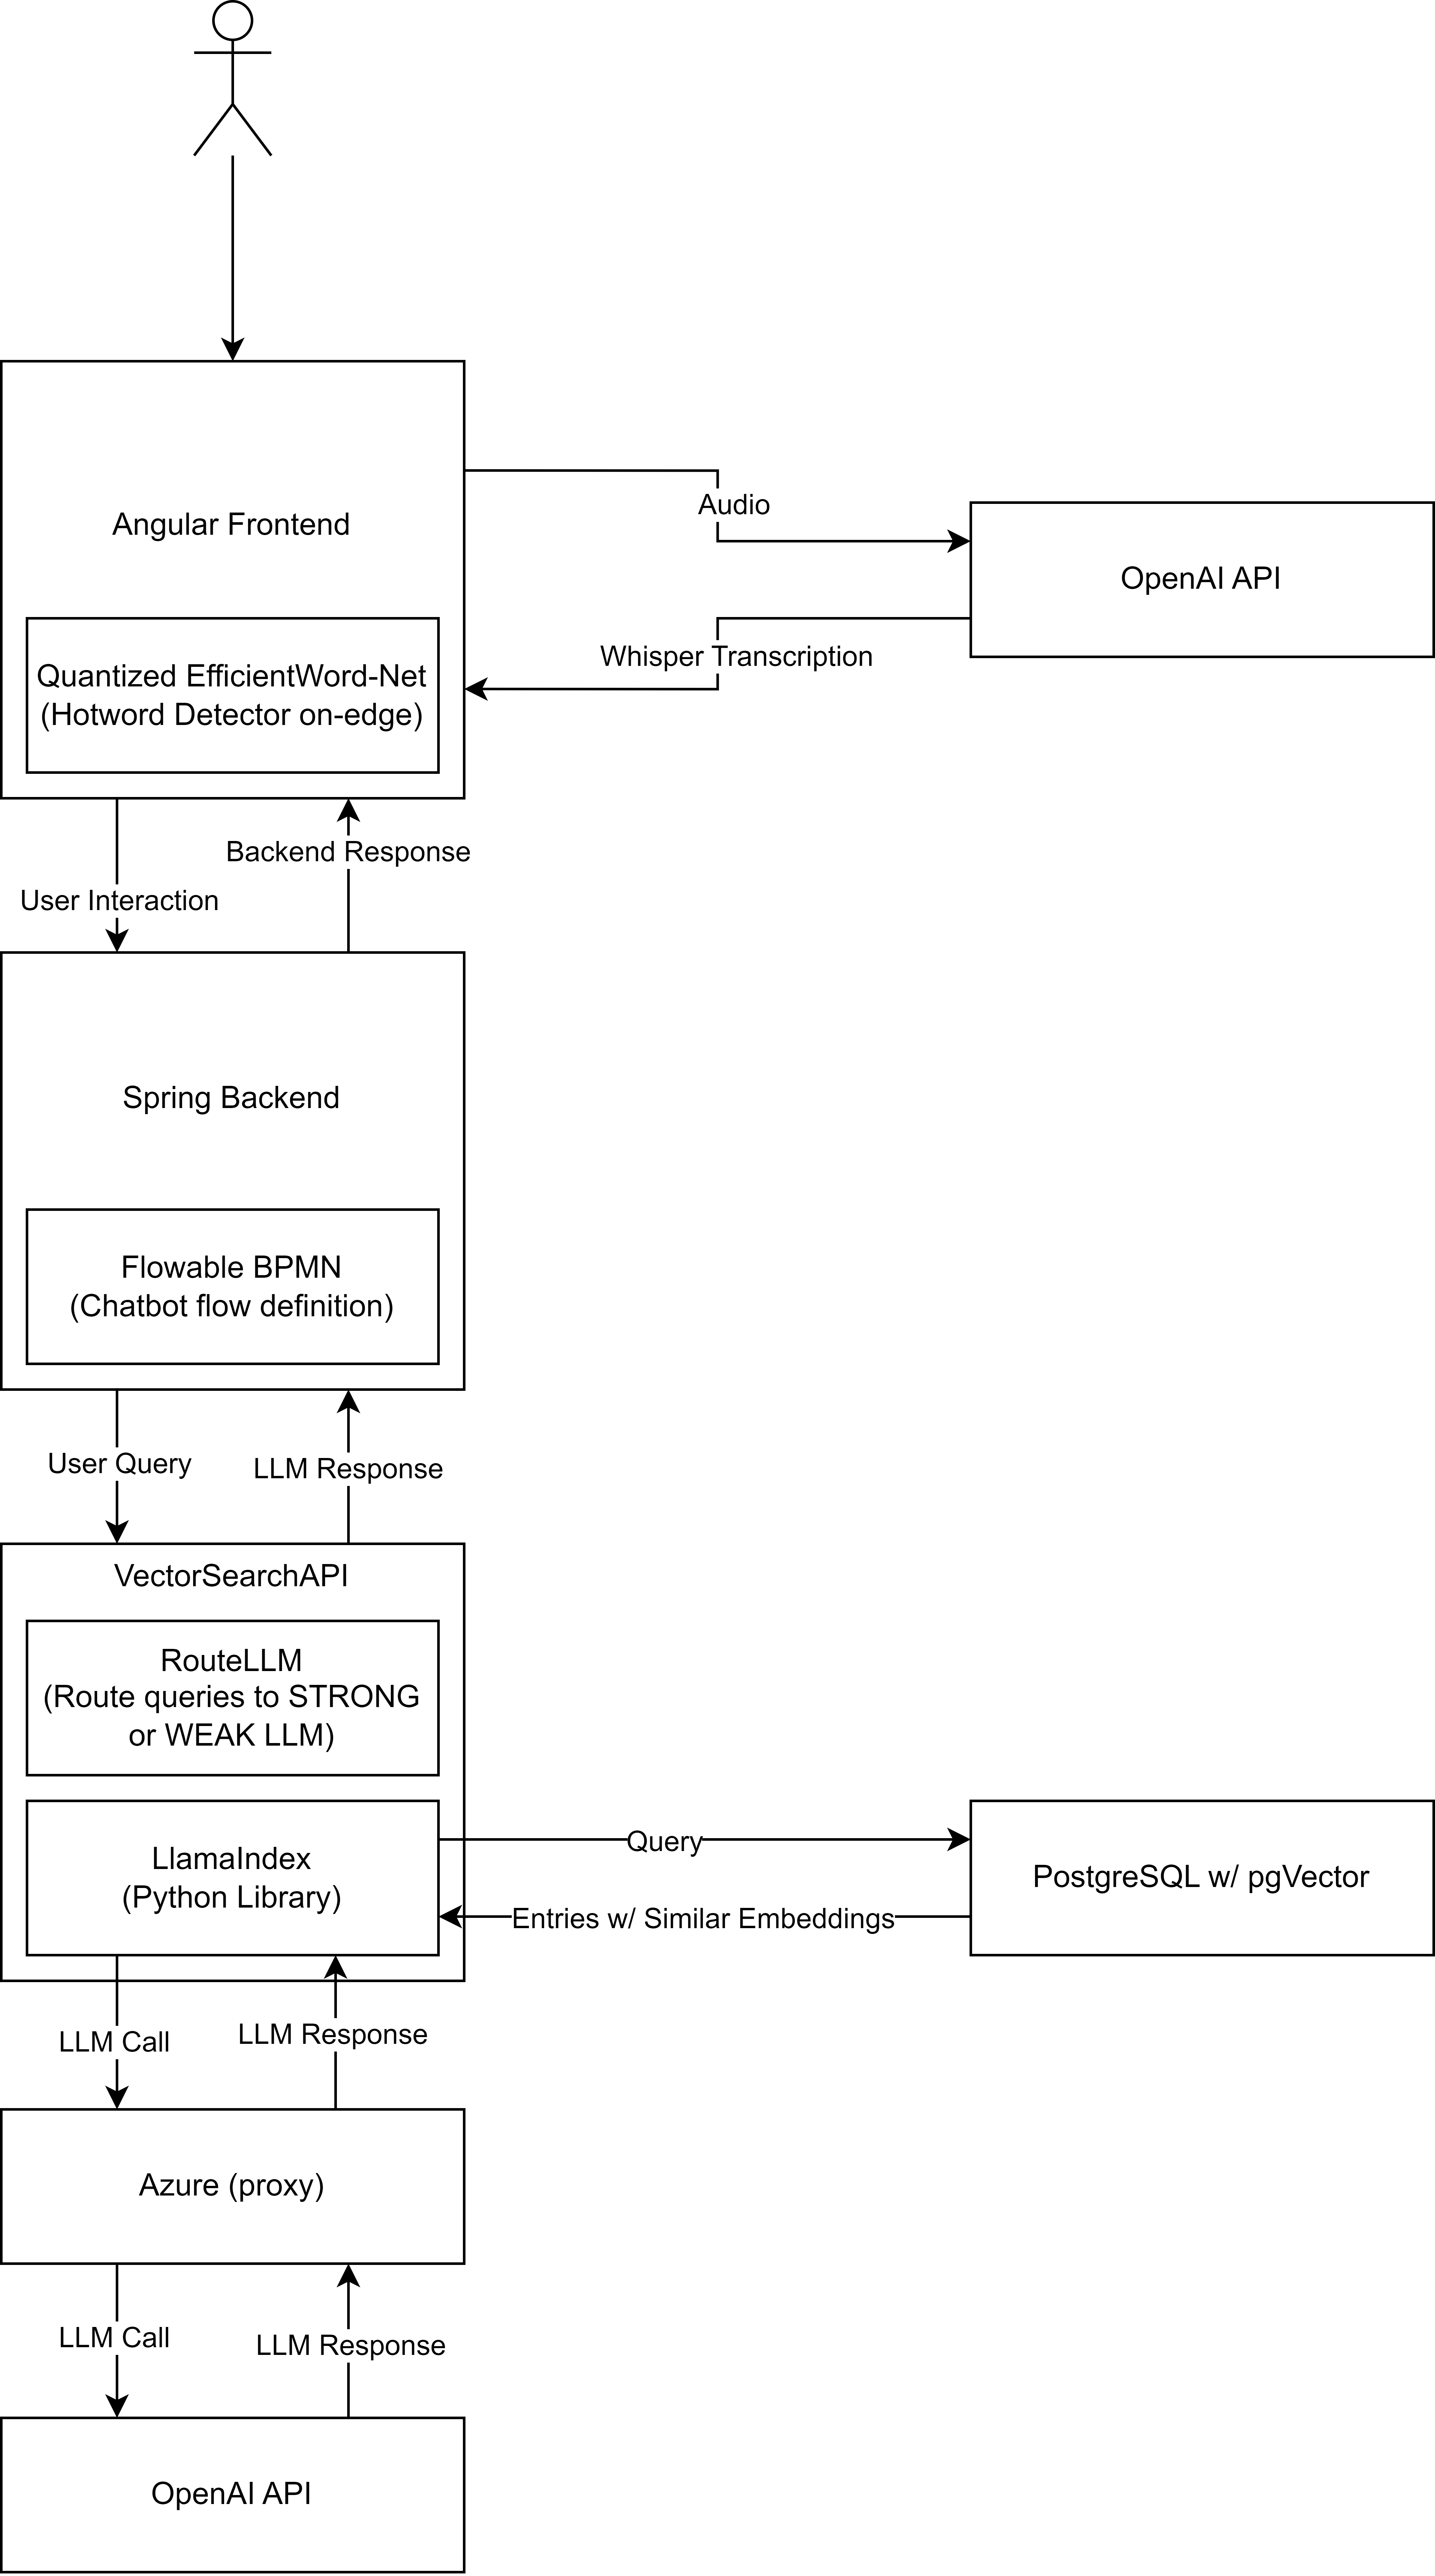
\includegraphics[width=1\textwidth]{imatges/Full DSO App Architecture.drawio.png}
\caption{App Architecture}
\end{figure}

Over the following sections we will describe the different components of the system in more detail, and how a user's interaction is processed through the system.

\subsection{Hotword/Wakeword Detection}
On the frontend we implement a custom version of the EfficientWord-Net \cite{Chidhambararajan2022EfficientWordNet} hotword detector, that has been quantized \cite{Zhang2023PostTrainingQuantizationNeuralNetworks}. To implement it we use ONNX \cite{onnx} and WebAssembly (Wasm) \cite{wasm}, which run directly in the browser, ensuring no data leaves the client's machine inadvertently. The hotword detector listens to the microphone data in real-time, and when it hears the keyword ``chat'' or ``chatbot'', it activates the microphone and starts recording. We will see how this data is processed in the \ref{subsec:azure_services} section.

The EfficientWord-Net model has been quantized to 8-bits, which has reduced the size of the model from 80MB to 20MB, and has improved the response time by 100\%. This has been achieved without perceptibly sacrificing the accuracy of the hotword detection.

The hotword detector analyzes audio data in chunks of 1.5 seconds, overlapped by 0.75 seconds. The raw audio signal is first converted to a Mel spectrogram (Figure~\ref{fig:mel_spectrogram}), which is then passed through a ResNet \cite{He2015DeepResidualLearningImage} model to generate semantic embedding vectors. These vectors are then compared to the embedding vectors of reference recordings of the hotword (which are prerecorded) using cosine similarity. If the similarity is above a certain threshold, the hotword is detected.
We use the pretrained model as provided by the EfficientWord-Net library, with no further training.

\begin{figure}[htb]
  \centering
  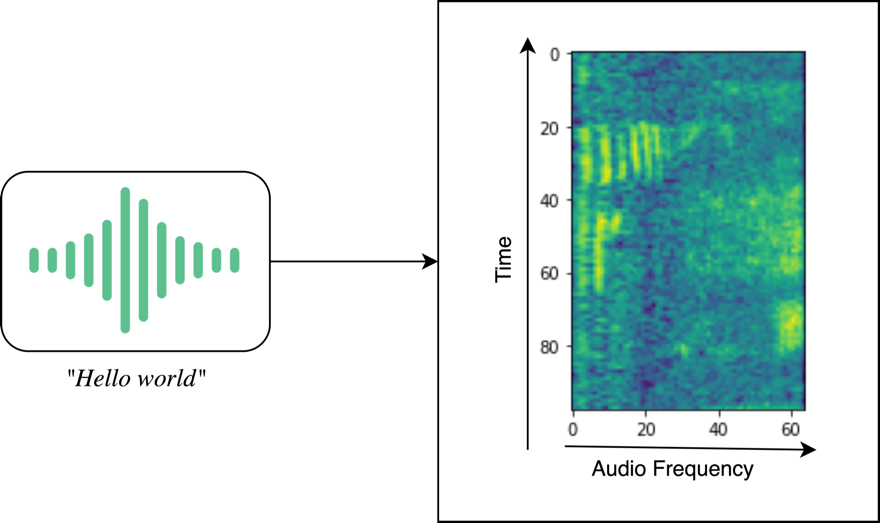
\includegraphics[width=1\textwidth]{imatges/MelSpectrogram.png}
  \caption{Mel spectrogram of the audio ``Hello world'' (image taken from \cite{Chidhambararajan2022EfficientWordNet})}
  \label{fig:mel_spectrogram}
\end{figure}

Because this system needs to run on the browser, and there is no existing implementation of a Mel spectrogram converter, we implement our own converter directly in TypeScript. This converter is as close as possible to a direct translation --from Python to TypeScript-- of the original code from the EfficientWord-Net library. By doing so we ensure data generated by our implementation is equivalent to that generated by the original implementation. We evaluate that this is the case by making bitwise comparisons of the output of both implementations (subtracting one image from the other), and find there are no differences (all pixels in the resulting image are exactly 0).

On our reference system, which consists of a Dell Latitude 3440 laptop with a 13th Gen Intel(R) Core(TM) i5-1345U CPU, the hotword detector has a response time of around 80-100 milliseconds, which is well within the acceptable range for real-time applications.

\subsection{Azure Services}
\label{subsec:azure_services}

\subsubsection{Speech-to-Text}

When the hotword detector activates the microphone, the audio data is sent to the Azure Speech-to-Text service. This service converts the audio data into text, which is then sent to the Backend for processing. The Azure Speech-to-Text service uses the Whisper \cite{Radford2022RobustSpeechRecognitionLargeScale} model to accurately transcribe speech into text.

\subsubsection{PostgreSQL Database}
\label{subsubsec:database}

The PostgreSQL database contains the text of the laws related to social rights and available social benefits in Catalonia. This data is indexed using the LlamaIndex Python library to chunk the text into smaller pieces, index them and  help create semantic embeddings. When a user query is received, the information retrieval system searches the database for the most relevant laws and benefits based on the query, and returns this information to the GPT model for generation.

\subsubsection{GPT Model}

The GPT model is used to generate coherent and contextually relevant responses to user queries based on the information retrieved from the database. The GPT model is a transformer-based \cite{Vaswani2023AttentionNeed} language model that is trained on a large dataset of text to generate human-like responses to user queries.

We use the GPT-4o and GPT-4o Mini models, which are the latest versions of the GPT model developed by OpenAI at the time of writing.

\subsection{Backend}

\subsubsection{Conversation Flow}

The Backend implements, among others, the conversation flow followed by the chatbot. It implements multiple stages and follows a state machine to manage the conversation. User queries at each stage are routed to the appropriate model.

Conversations flows are implemented using Flowable. Here are the flow diagrams for the conversation stages:


\begin{figure}[htb]
  \label{fig:conversation}
  \centering
  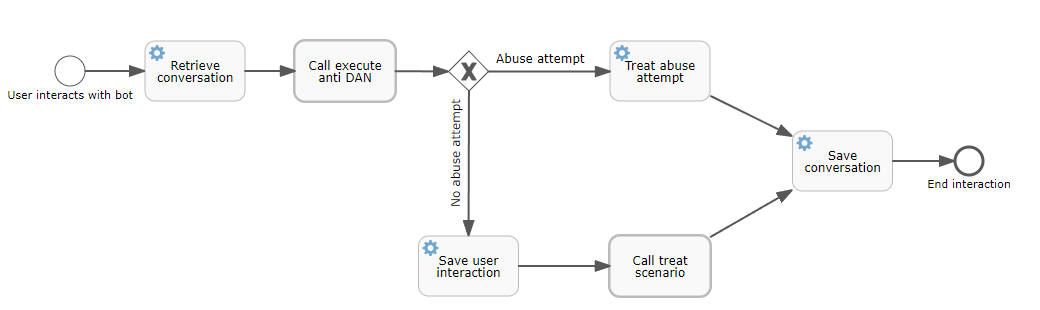
\includegraphics[width=1\textwidth]{imatges/0_DsoConversation.png}
  \caption{Top level flow diagram for the conversation}
\end{figure}

\begin{figure}[htb]
  \centering
  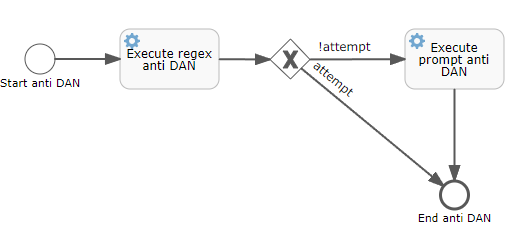
\includegraphics[width=1\textwidth]{imatges/1_DsoExecuteAntiDAN.png}
  \caption{Flow diagram for the Anti DAN stage}
  \label{fig:antidan}
\end{figure}

\begin{figure}[htb]
  \centering
  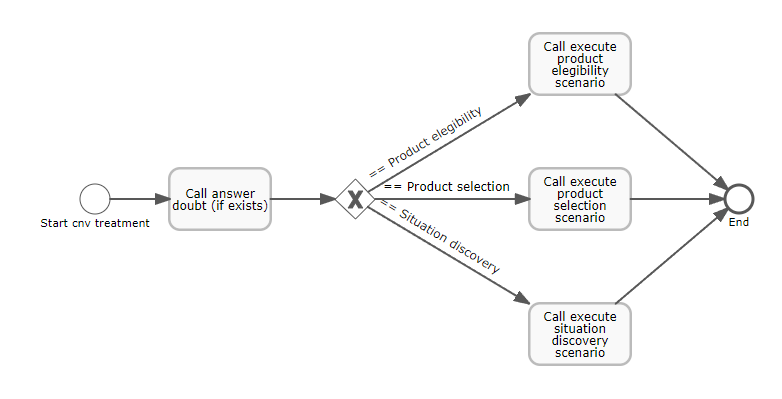
\includegraphics[width=1\textwidth]{imatges/2_DsoTreatScenario.png}
  \caption{Flow diagram for the Treat Scenario stage}
\end{figure}

\begin{figure}[htb]
  \centering
  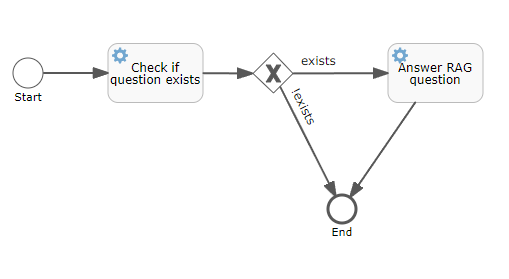
\includegraphics[width=1\textwidth]{imatges/3_AnswerRagQuestionIfExists.png}
  \caption{Flow diagram for the Answer RAG Question If Exists stage}
\end{figure}

\begin{figure}[htb]
  \centering
  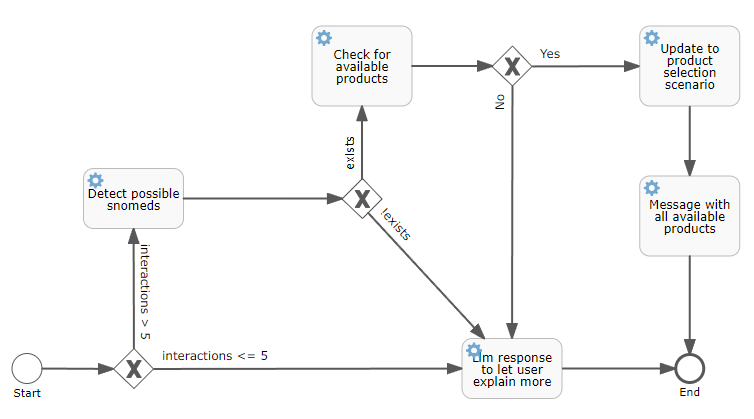
\includegraphics[width=1\textwidth]{imatges/4_1_DsoExecuteSituationDiscoveryScenario.png}
  \caption{Flow diagram for the scenario where we need to discover the user's situation}
\end{figure}

\begin{figure}[htb]
  \centering
  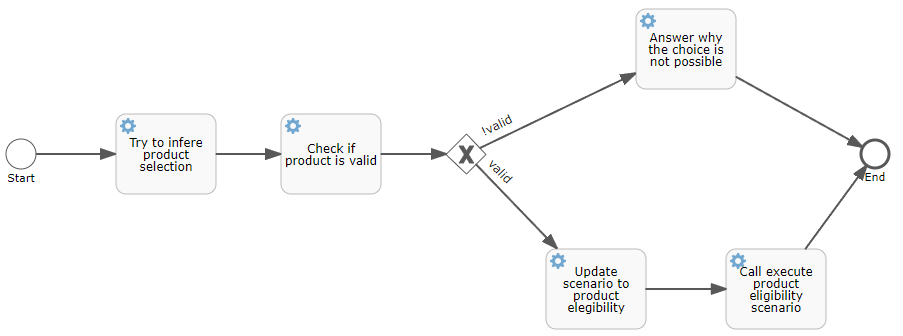
\includegraphics[width=1\textwidth]{imatges/4_2_DsoExecuteProductSelectionScenario.png}
  \caption{Flow diagram for the scenario where we need to select a product from the kSocial catalog given the conversation we have had with the user}
\end{figure}

\begin{figure}[htb]
  \centering
  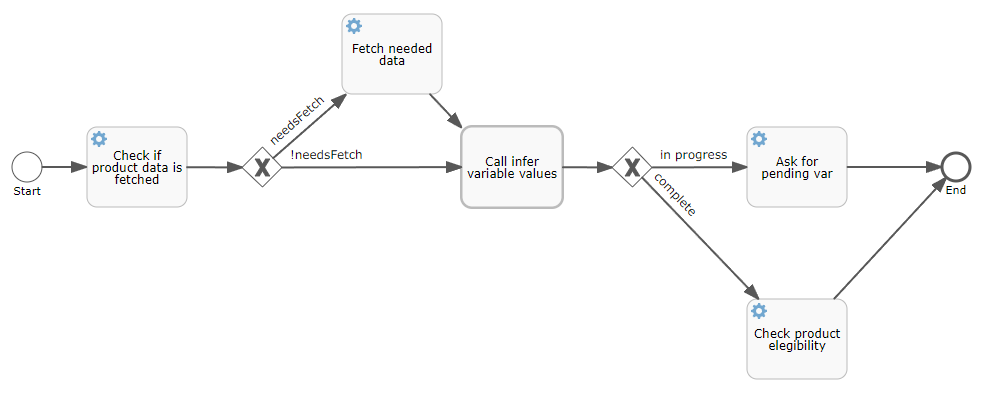
\includegraphics[width=1\textwidth]{imatges/4_3_DsoProductElegibilityScenario.png}
  \caption{Flow diagram for the scenario where we need the user to select one of the products from the kSocial catalog}
\end{figure}

\begin{figure}[htb]
  \centering
  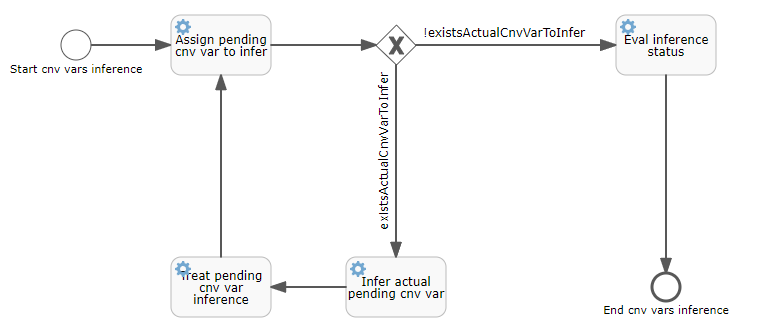
\includegraphics[width=1\textwidth]{imatges/5_InferVariablesProcess.png}
  \caption{Flow diagram for inferring necessary variables for the current scenario based on the conversation}
\end{figure}



\subsubsection{Model Routing}

We use a slightly tweaked version of the fairly new RouteLLM python library. This allows us to route a certain percentage of queries to a "stronger", more expensive model and the rest to a "weaker", less expensive model. With this system we are able to achieve X\% of the performance of the stronger model at a fraction of the cost. The RouteLLM system uses a small BERT classifier model that decides which queries should be routed to the stronger model and which to the weaker model. This classifier was trained by the original library authors on a dataset of human preferences augmented with synthetic data generated using GPT-4. They report good generalization performance, so we apply the system on a pair consisting of GPT-4o and GPT-3.5-Turbo.

// TODO: PUT HERE EXAMPLES OF CONVERSATIONS BEING ROUTED TO DIFFERENT MODELS DEPENDING ON WHAT IS BEING ASKED.


\subsubsection{Information Retrieval}

We do RAG using the LlamaIndex python library. We use a less common RAG algorithm that uses hierarchical embeddings of chunks, allowing us to capture both fine-grained and coarse-grained information. We call this method "Small To Big Retrieval" or STBR.

\subsection{Our Contributions}
During the development of this project we have iterated and made changes to a few existing tools and components. Here we link to our forks of the repositories.

\begin{itemize}
  \item EfficientWord-Net: \url{https://github.com/SupremeLobster/EfficientWord-Net} - Our fork of the EfficientWord-Net library, which has been modified to reduce response time, client machine requirements, and the size of downloaded files, through Quantization methods.
  \item RouteLLM: \url{https://github.com/SupremeLobster/RouteLLM} - Our fork of the RouteLLM library, which allows us to route a certain percentage of queries to a "stronger", more expensive model and the rest to a "weaker", less expensive model. Our changes are in the branch "feature/support-azure-openai-embeddings". These changes made the library compatible with the Azure OpenAI models, which didn't have official support.
\end{itemize}

\chapter{Estat de l'art}
\label{cap:estat}

\section{Secció}

\subsection{Subsecció}

\chapter{Preliminars}
\label{cap:prelim}

\chapter{Planificació i Metodologia}
\label{cap:plan}

\chapter{Contribució Metodològica}
\label{cap:contrib}

\chapter{Resultats}
\label{cap:result}

\chapter{Conclusions i treball futur}
\label{cap:concl}

\backmatter

%\appendix

%\include{Appendix1}

% \bibliographystyle{ThesisStyleBreakable}
\bibliographystyle{ieeetr}
\bibliography{biblio}

%\printnomenclature

\end{document}
